\usetikzlibrary{arrows.meta}
\tikzset{
  exam conic edge/.style={line width=.6pt},
  exam conic curve/.style={line width=.6pt},
  exam conic axis/.style={line width=.6pt,>=Stealth},
  exam conic label/.style={inner sep=0pt,outer sep=0pt,font=\normalsize}
}
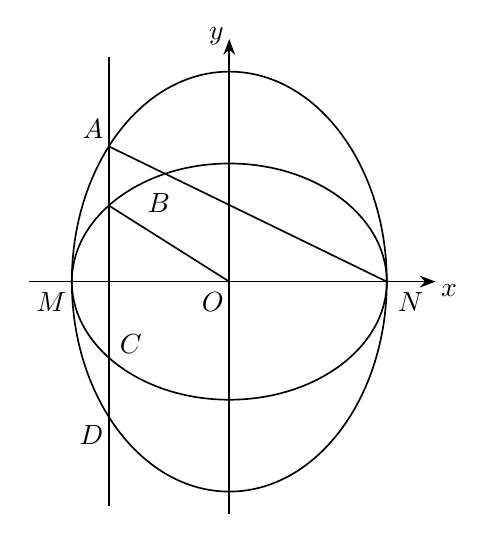
\begin{tikzpicture}[x=1cm,y=1cm,line width=.6pt,font=\normalsize,>=Stealth]
\coordinate (O) at (0,0);
\coordinate (M) at (-2,0);
\coordinate (N) at (2,0);
\coordinate (A) at (-1.53,1.717414077);
\coordinate (B) at (-1.53,0.966045418);
\coordinate (C) at (-1.53,-0.966045418);
\coordinate (D) at (-1.53,-1.717414077);
\coordinate (Lbottom) at (-1.53,-2.85);
\coordinate (Ltop) at (-1.53,2.85);
\coordinate (Xleft) at (-2.55,0);
\coordinate (Xright) at (2.62,0);
\coordinate (Ydown) at (0,-2.95);
\coordinate (Yup) at (0,3.08);
\draw[exam conic curve] (O) ellipse [x radius=2cm, y radius=2.666666667cm];
\draw[exam conic curve] (O) ellipse [x radius=2cm, y radius=1.5cm];
\draw[exam conic edge] (Lbottom)--(Ltop);
\draw[exam conic edge] (A)--(N);
\draw[exam conic edge] (B)--(O);
\draw[exam conic axis,->] (Xleft)--(Xright);
\draw[exam conic axis,->] (Ydown)--(Yup);
\node[exam conic label,below left,xshift=-2pt,yshift=-4pt] at (M) {$M$};
\node[exam conic label,below right,xshift=4pt,yshift=-4pt] at (N) {$N$};
\node[exam conic label,below left,xshift=-2pt,yshift=-4pt] at (O) {$O$};
\node[exam conic label,above left,xshift=-2pt,yshift=3pt] at (A) {$A$};
\node[exam conic label,right,xshift=14pt,yshift=1pt] at (B) {$B$};
\node[exam conic label,right,xshift=4pt,yshift=5pt] at (C) {$C$};
\node[exam conic label,below left,xshift=-2pt,yshift=-3pt] at (D) {$D$};
\node[exam conic label,below right,xshift=2pt,yshift=-1pt] at (Xright) {$x$};
\node[exam conic label,left,xshift=-2pt,yshift=1pt] at (Yup) {$y$};
\end{tikzpicture}
